\subsection{Shifted Parabolas on the Branches}
\label{sec:setup.quad.skewed}

\hl{
	The choice of centering the parabola-shaped branches was not ideal.
}
When looking at the original model function, one can see that the parabolas are not centered.
All branches are more shifted to the left.
To imitate this shape better, \hl{the parameters are} set to $b_L = -\frac{1}{2}$ and $b_R = -\frac{7}{2}$ \hl{in this section}.
All other fixed parameters are the same as \hl{in the previous section,} \Cref{sec:setup.quad.even}.
The parameters $c_L$ and $c_R$ are varied in the intervals $[0.08, 0.525]$ and $[0.825, 1.275]$, respectively.

\hl{
	With the newly chosen fixed parameter values, this model imitates the shape of the original model function better.
	And it perfectly emulates the effects of $\chi_0$ on the branches $F_\A$ and $F_\C$ of the original model function still, as described in the previous section.
	But it still does not emulate the effects of the parameter $E_0$ on the branches $F_\B$ and $F_\D$ of the original model function.
}

\Cref{fig:setup.quad.skew.period.full} shows a 2D scan of the periods \hl{associated with the parameter regions} in this parameter range.
The structure seen in this figure repeats \hl{infinitely} in all directions.
An interesting parameter \hl{range} is marked with a red rectangle.
In this parameter \hl{range}, 2 wings with the \hl{same} period connect.
\hl{
	In the previous section this was not the case and that was one reason for rejecting that model.
}
\Cref{fig:setup.quad.skew.period.zoomed} shows a 2D scan of the periods \hl{associated with the parameter regions in} this parameter range.
The points indicate the parameter values \hl{used} for the \hl{analysis with cobweb diagrams}.

\begin{figure}
	\centering
	\begin{subfigure}{0.4\textwidth}
		\centering
		\includegraphics[width=\textwidth]{21_Quadratic_mod1/Skew/2D_Period_SZoomed1/result.png}
		\caption{Full}
		\label{fig:setup.quad.skew.period.full}
	\end{subfigure}
	\begin{subfigure}{0.4\textwidth}
		\includegraphics[width=\textwidth]{21_Quadratic_mod1/Skew/2D_Period_SZoomed2/result.png}
		\caption{Zoomed}
		\label{fig:setup.quad.skew.period.zoomed}
	\end{subfigure}
	\caption[2D scans showing periods of the skewed piecewise quadratic model]{
		2D scans showing the periods of the piecewise quadratic model with fixed parameters $a_L = a_R = 6$, $b_L = -\frac{1}{2}$, and $b_R = -\frac{7}{2}$.
		(a) Shows the full structure with parameters $c_L$ and $c_R$ being varied in the ranges $[0.08, 0.525]$ and $[0.825, 1.275]$, respectively.
		The red rectangle marks the parameter range \hl{is shown magnified in} (b).
		The marked points in (b) are the parameter values for the \hl{cobweb diagrams} in \Cref{fig:setup.quad.skew.cobwebs}
	}
	\label{fig:setup.quad.skew.period}
\end{figure}

\begin{figure}
	\centering
	\subfloat[At point $A$]{
		\includegraphics[width=.3 \textwidth]{21_Quadratic_mod1/Skew/Cobweb_SA/result.png}
		\label{fig:setup.quad.skew.cobweb.A}
	}
	\subfloat[At point $B$]{
		\includegraphics[width=.3 \textwidth]{21_Quadratic_mod1/Skew/Cobweb_SB/Manual/result.png}
		\label{fig:setup.quad.skew.cobweb.B}
	}
	\subfloat[At point $C$]{
		\includegraphics[width=.3 \textwidth]{21_Quadratic_mod1/Skew/Cobweb_SC/result.png}
		\label{fig:setup.quad.skew.cobweb.C}
	}
	\caption[Cobwebs of the skewed piecewise quadratic model]{
		Cobweb diagrams at three parameter values of $c_L$ and $c_R$ in the piecewise quadratic model with fixed parameters $a_L = a_R = 6$, $b_L = -\frac{1}{2}$, and $b_R = -\frac{7}{2}$.
		The parameter values are marked in \Cref{fig:setup.quad.even.period.zoomed}.
		(a) shows the cycle $\Cycle{\A^3\B^3\C^3\D^3}$ at point $A$ \hl{where $c_L = 0.1385$ and $c_R = 0.925$},
		(b) shows the two coexisting cycles $\Cycle{\A^3\B^3\C^3\D^3}$ (green) and $\Cycle{\A^4\B^2\C^4\D^2}$ (red) at point $C$ \hl{where $c_L = 0.141$ and $c_R = 0.911$},
		and (c) shows the cycle $\Cycle{\A^4\B^2\C^4\D^2}$ \hl{where $c_L = 0.142$ and $c_R = 0.9095$}.
	}
	\label{fig:setup.quad.skew.cobwebs}
\end{figure}

\Cref{fig:setup.quad.skew.cobwebs} shows all the \hl{cobweb diagrams of the model at with the parameter values marked} in \Cref{fig:setup.quad.skew.period.zoomed}.
The cobweb at point $A$ is shown in \Cref{fig:setup.quad.skew.cobweb.A}.
\hl{One} can see that it has period 12 and its symbolic sequence is $\A^4\B^2\C^4\D^2$.
The cycle at point $C$ also has period 12.
Its cobweb diagram is shown in \Cref{fig:setup.quad.skew.cobweb.C}, and \hl{one} can see that its symbolic sequence is $\A^3\B^3\C^3\D^3$.

From point $A$ to point $C$, one point of the cycle on the branch $f_\A$ moved to the branch $f_\B$.
The same thing happened to a point of the cycle on the branch $f_\C$, it moved to the branch $f_\D$.
This is similar to what happens in the original model along a chain of parameter regions with the same period.
And in between both points, there is a parameter region where 2 cycles coexist.
This is shown in \Cref{fig:setup.quad.skew.cobweb.B}, which depicts the cycles at point $C$.
But unfortunately, the coexisting cycles are the same cycles that exist at point $A$ and point $C$, $\Cycle{\A^4\B^2\C^4\D^2}$ and $\Cycle{\A^3\B^3\C^3\D^3}$.
Similarly to the previous \hl{experiment}, we merely observe two parameter regions with stable cycles overlapping.
